\section{CNN}
$\varphi(W * v^{(l)})$ 
For each channel there is a separate filter.

\subsection*{Convolution}
    $C = channel$ $F = filterSize$ $inputSize = I$ $padding = P$
    $stride = S$ \\
$ \text{Output size l} = \frac{I + 2P - K}{S} + 1$\\
    $\text{Output dimension} = l \times l \times m $\\
    $\text{Inputs} = W * H * D * C * N $\\
    $\text{Trainable parameters} = F * F * C * \# filters$
\section*{Neural Networks, d.o.i}
$w$ are the weights and $\varphi: \R \mapsto \R$ is a nonlinear \textbf{activation function}: $\phi(x, w) = \varphi(w^\top x)$


$\textbf{ReLU: } \max (0,z), \; \textbf{Tanh: } \frac{\exp(z) - \exp(-z)}{\exp(z) + \exp(-z)}$ \\[-3pt]
$\textbf{Sigmoid: } \frac{1}{1 + \exp(-z)}$


\textbf{Universal Approximation Theorem}: We can approximate any arbitrary smooth target function, with 1+ layer with sufficient width.

\subsection*{Forward Propagation}

Input: $v^{(0)} = [x; 1]$ \quad Output: $f = W^{(L)} v^{(L-1)}$
Hidden: $z^{(l)} = W^{(l)} v^{(l-1)}, v^{(l)} = [\varphi(z^{(l)}); 1]$


\subsection*{Backpropagation}

Non-convex optimization problem: 

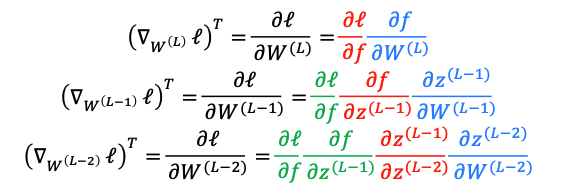
\includegraphics[width=\columnwidth]{jo/backpropagation.png} \\[-10pt]

Only compute \textbf{the gradient}. Rand. init. weights by distr. assumption for $\varphi$. ( $2 / n_{in}$ for ReLu and $1/n_{in}$ or $ 1/ (n_{in} + n_{out})$ for Tanh)

\subsection*{Gradient Descent, i.o.i}
Converges only for convex case. $\mathcal{O}(n * k * d)$
$$
	w^{t+1} = w^t - \eta_t \cdot \nabla \ell(w^t)
$$

For linear regression:
$$
	||w^t - w^*||_2 \leq ||I - \eta X^\top X||_{op}^t ||w^0 - w^*||_2
$$

$\rho = ||I - \eta X^\top X||_{op}^t$ conv. speed for const. $\eta$. Opt. fixed $\eta = \frac{2}{\lambda_{\text{min}} + \lambda_{\text{max}}}$ and max. $\eta \leq \frac{2}{\lambda_{\text{max}}}$. 

\textbf{Momentum}: $w^{t+1} = w^t + \gamma \Delta w^{t-1} - \eta_t \nabla \ell(w^t)$
Learning rate $\eta_t$ guarantees convergence if $\sum_t \eta_t = \infty$ and $\sum_t \eta_t^2 < \infty$
